
\subsection{Esercizio circuito magnetico}
Si realizza un circuito magnetico come in figura
\begin{figure}[H]
\centering
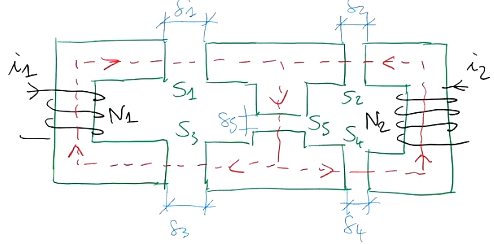
\includegraphics[width = 0.5\linewidth]{esercizio_circuito_magnetico}
\end{figure}

Si vogliono determinare i coefficienti di auto e mutua induzione del circuito, i dati
sono:
$$
\begin{aligned}
&N_1 = 400 \qquad N_2 = 200\\
&\delta_1 = \delta_3 = \SI{2}{\milli\meter}\\
&\delta_2=\delta_4 = \SI{3}{\milli\meter} \\
&\delta_5 = \SI{5}{\milli\meter}\\
&S_1 = S_2 = S_3 = S_4 = S_\delta = \SI{25}{\milli\meter^2}
\end{aligned}
$$
Orientati i flussi si può realizzare l'equivalente circuitale
\begin{figure}[H]
\centering
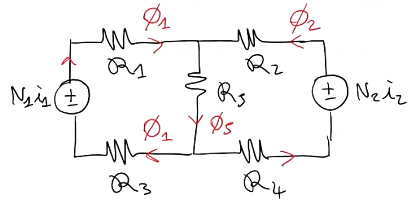
\includegraphics[width = 0.4\linewidth]{esercizio_circuito_magnetico_equivalente_resistivo}
\end{figure}
Si calcolano le riluttanze
$$\begin{aligned}
&\mathcal{R}_1 = \frac{\delta_1}{\mu_0 S} = \mathcal{R}_3 = \frac{\SI{2e-3}{}}{\mu_0\cdot\SI{25e-6}{}} = \SI{6.37e7}{\henry^{-1}}\\
&\mathcal{R}_2 = \frac{\delta_2}{\mu_0S} = \mathcal{R}_4 = \frac{\SI{3e-3}{}}{\mu_0\cdot\SI{25e-6}{}} = \SI{9.55e7}{\henry^{-1}}\\
&\mathcal{R}_5 = \frac{\delta_5}{\mu_0S} = \frac{\SI{5e-3}{}}{\mu_0\cdot\SI{25e-6}{}} = \SI{15.9e7}{\henry^{-1}}\end{aligned}
$$
\newpage
I flussi concatenati da calcolare sono 
$$
\begin{aligned}
&\Phi_1^c = N_1\Phi_1\\
&\Phi_2^c = N_2\Phi_2
\end{aligned}
$$
e quindi i coefficienti di auto e mutua induzione
$$
\begin{aligned}
L_1 &= \left.\frac{\Phi_1^c}{i_1}\right|_{i_2=0} = \frac{N_1\Phi_1'}{i_1}\\
M_{21} &= \left.\frac{\Phi_2^c}{i_1}\right|_{i_2=0} = \frac{N_2\Phi_2'}{i_1}
\end{aligned}
$$
I flussi si calcolano ricavando la riluttanza equivalente ed eseguendo un partitore
di corrente
$$
\begin{aligned}
\Phi_1' &= \frac{N_1i_1}{\mathcal{R}_1+\mathcal{R}_3+\mathcal{R}_5//\left(\mathcal{R}_2+\mathcal{R}_4\right)}\\
\Phi_2' &= -\Phi_1' \frac{\mathcal{R}_5}{\mathcal{R}_5+\mathcal{R}_2+\mathcal{R}_4}
\end{aligned}
$$
quindi
$$
\begin{aligned}
L_1 &= \frac{N_1^2}{\mathcal{R}_1 + \mathcal{R}_3 + \mathcal{R}_5//\left(\mathcal{R}_2+\mathcal{R}_4\right)} = \SI{0.48}{\milli\henry}\\
M_{21} &= -\frac{N_2N_1}{\mathcal{R}_1+\mathcal{R}_3+\mathcal{R}_5//\left(\mathcal{R}_2+\mathcal{R}_4\right)}\cdot\frac{\mathcal{R}_5}{\left(\mathcal{R}_5+\mathcal{R}_2+\mathcal{R}_4\right)} = \SI{-0.17}{\milli\henry}
\end{aligned}
$$
Per calcolare ora l'auto-induttanza $L_2$ è necessario spegnere il primo generatore
ma si vede che il circuito è topologicamente simmetrico, dunque si possono sostituire
i valori delle riluttanze corretti nelle relazioni precedenti.
$$\begin{aligned}
\Phi_2'' &= \frac{N_2i_2}{\mathcal{R}_2+\mathcal{R}_4+\mathcal{R}_5//\left(\mathcal{R}_1+\mathcal{R}_3\right)}\\
\Phi_1'' &= -\Phi_2'' \frac{\mathcal{R}_5}{\mathcal{R}_5 + \mathcal{R}_1+\mathcal{R}_3}
\end{aligned}
$$
$$
\begin{aligned}
L_2 &= \frac{N_2^2}{\mathcal{R}_2 + \mathcal{R}_4 +\mathcal{R}_5//\left(\mathcal{R}_1+\mathcal{R}_3\right)} = \SI{0.15}{\milli\henry}\\
M_{12} &= - \frac{N_1N_2}{\mathcal{R}_2+\mathcal{R}_4+\mathcal{R}_5//\left(\mathcal{R}_1+\mathcal{R}_3\right)}\cdot\frac{\mathcal{R}_5}{\left(\mathcal{R}_5+\mathcal{R}_1+\mathcal{R}_3\right)} = \SI{-0.17}{\milli\henry}
\end{aligned}
$$
$M_{12}=M_{21}$ per la reciprocità.

\newpage
\section{Modelli quasi-stazionari dell'elettromagnetismo}
Si suppone che le sorgenti varino nel tempo ma i tempi caratteristici delle variazioni
siano ``sufficientemente lunghi''.
Si richiamano le equazioni di Maxwell
$$
\begin{aligned}
&\oiint_\Sigma\vec{B}\cdot\hat{n}dS = 0\ \ \forall\ \Sigma \text{ chiusa di } \mathbb{R}^3\\
&\oiint_\Sigma\vec{D}\cdot\hat{n}dS = Q_{\text{lib }\Omega_\Sigma} \\
&\oint_\Gamma \vec{E}\cdot\hat{t} dl = - \iint_{S_\gamma} \frac{\partial\vec{B}}{\partial t}\cdot\hat{n}dS \ \ \forall\ \Gamma \text{ chiusa di } \mathbb{R}^3\\
&\oint_\Gamma \vec{H}\cdot\hat{t}dl = i_\Gamma + \iint_{S_\Gamma} \frac{\partial\vec{D}}{\partial t}\cdot\hat{n} dS\\
&\oiint_\Sigma \vec{J}_\text{lib} \cdot\hat{n}dS = - \iiint_{\Omega_\Sigma} \frac{\partial \rho_\text{lib}}{\partial t}dV\ \ \forall\ \Sigma \text{ chiusa di }\mathbb{R}^3
\end{aligned}
$$
Le ultime tre di queste equazioni contengono delle variazioni nel tempo delle grandezze, queste
grandezze sono legate tra loro ma se si suppone di poterle far variare
in maniera indipendente istante per istante. 

Si sviluppano dunque modelli differenti, il primo
se si suppone che resti costante il vettore spostamento $\vec{D}$, prende il nome
di ``Magneto-Quasi-Stazionario'' (MQS) in cui i campi magnetici si determinano a partire dalla
conoscenza delle distribuzioni di corrente e i campi elettrici si ricavano a posteriori.

Il secondo modello che prende il nome di ``Elettro-Quasi-Stazionario'' (EQS) in cui si 
trascura la variazione del campo di induzione magnetica e vale solitamente per i 
dielettrici.

Un terzo modello che generalizza la conduzione stazionaria prende il nome di
``rilassamento della carica'' sempre trascurando la variazione del campo di induzione
magnetica $\vec{B}$, equivale al modello EQS in presenza di conduttori.

Riassumendo
\begin{enumerate}
\item MQS $\rightarrow \frac{\partial\vec{D}}{\partial t},\ \frac{\partial \rho_\text{lib}}{\partial t} \simeq 0$
\item EQS $\rightarrow\frac{\partial\vec{B}}{\partial t} \simeq 0 $ (dielettrici)
\item Rilassamento della carica $\frac{\partial\vec{B}}{\partial t} \simeq 0$ (conduttori)
\end{enumerate}

Si analizza il modello del rilassamento della carica, in forma locale. Si suppone
di avere un certo dominio $\Omega$ che si comporta sia da conduttore che da dielettrico,
caratterizzato dunque da una conducibilità $\gamma$ e una permittività dielettrica
$\varepsilon$ costanti.

Le equazioni di Maxwell in forma locale diventano:
$$
\begin{aligned}
&\text{Nei punti regolari}\\
&\nabla\cdot\vec{D} = \rho_\text{lib} \\
&\nabla\times\vec{E} = 0\\
&\nabla\cdot\vec{J}_\text{lib} = -\frac{\partial \rho_\text{lib}}{\partial t}
\end{aligned}\qquad 
\begin{aligned}
&\text{Sulle superfici di discontinuità e.g. }\partial \Omega\\
&\hat{n}\cdot\left(\vec{D}_2-\vec{D}_1\right) = \sigma_\text{lib}\\
&\hat{n}\times\left(\vec{E}_2-\vec{E}_1\right) = 0\\
&\hat{n}\cdot\left(\vec{J}_2-\vec{J}_1\right) = -\frac{\partial\sigma_\text{lib}}{\partial t}
\end{aligned}
$$
A queste si aggiungono le relazioni costitutive
$$
\begin{aligned}
&\vec{D} = \varepsilon\vec{E}\\
&\vec{J}_\text{lib} = \gamma \vec{E}
\end{aligned}
$$
Sostituendo nelle equazioni di Maxwell
$$
\vec{D} = \varepsilon\frac{\vec{J}_\text{lib}}{\gamma} \Rightarrow \nabla\cdot\left(\frac{\varepsilon}{\gamma}\vec{J}_\text{lib}\right) = \rho_\text{lib}=
\frac{\varepsilon}{\gamma}\nabla\cdot\vec{J}_\text{lib} = \frac{\varepsilon}{\gamma}\left(-\frac{\partial \rho_\text{lib}}{\partial t}\right)
$$

questo implica che 
$$
\tau_e \frac{\partial\rho_\text{lib}}{\partial t} + \rho_\text{lib} = 0
$$
con $\tau_e = \frac{\varepsilon}{\gamma}$ che rappresenta il tempo di rilassamento della
carica libera in un conduttore omogeneo.

La precedente è un'equazione differenziale a derivate parziali dato che $\rho_\text{lib}$
è funzione del tempo ma anche del punto $p'$, la sua soluzione generale è
$$
\rho_\text{lib}(p',t) = \rho_\text{lib}(p',t=0)e^{-\frac{t}{\tau_e}}
$$
dove il termine per $t=0$ è la distribuzione di carica iniziale.

L'equazione vale indipendentemente da ciò che accade nel dominio $\Omega$ ossia in un 
conduttore omogeneo la carica libera si distribuisce sulla superficie di frontiera $\partial\Omega$ in un tempo pari a $(4\div 5)\ \tau_e$.
Sul conduttore non sono presenti dunque distribuzioni di cariche libere di volume ma 
solo distribuzioni di cariche superficiali.

Se le variazioni delle sorgenti sono molto più lente di $\tau_e$ è possibile applicare
il modello di corrente quasi-stazionaria.
\newpage
\subparagraph{Esempio numerico}
$$
\varepsilon = \varepsilon_r\varepsilon_0,\qquad \varepsilon_0 = \SI{8.85e-12}{\farad\per\meter}
$$
$$
\gamma = 
\begin{cases}
\gamma_{Cu} &\simeq \SI{e7}{\siemens\per\meter}\\
\gamma_{H_2O} &\simeq \SI{e-4}{\siemens\per\meter}
\end{cases}
$$
\begin{table}[H]\centering
\begin{tabular}{|c|c|c|c|}
 \hline Materiale & $\gamma[\si{\siemens\per\meter}]$ & $\varepsilon_r$ & $\tau_e[\si{\second}]$ \\
 \hline  &                                          &               &               \\
 $Cu$        & $\SI{5.8e7}{}$                    &   1           &   $\SI{1.5e-19}{}$ \\ 
 $H_2O$           & $\SI{2e-4}{} $                   &       81         & $\SI{3.6e-6}{}$ \\  
 Mica               & $\SI{e-11}{}\div\SI{e-15}{}$       &  5.8        &   $\SI{5.1}{}\left(1\div\SI{e4}{}\right)$ \\ \hline
\end{tabular}
\end{table}

Nel caso in cui il materiale non fosse omogeneo, l'analisi risulterebbe troppo complessa per gli
obbiettivi del corso e non verrà trattata. Si suppone invece che i materiali siano sempre almeno 
omogenei a tratti.

\paragraph{Modello Quasi-Stazionario-Magnetico MQS}
$\frac{\partial\vec{D}}{\partial t} \to 0$, $\frac{\partial\rho_\text{lib}}{\partial t}\to 0$
Si suppone che ci sia una distribuzione di correnti assegnate in una certa regione causa
di un campo di induzione magnetica $\vec{B}$ nello spazio per la legge di Biot-Savart.

Si vuole estendere questo fenomeno a correnti variabili nel tempo in maniera quasi stazionaria
affinché non ci siano correnti di spostamento
1:00:00
